\documentclass[nocolor]{tudbook}
\usepackage{tudthesis, german}
\usepackage[utf8]{inputenc}
\usepackage{bibgerm}
\usepackage{url}
\usepackage{paralist}

\urldef{\GitHubDesktop}\url{https://assets-cdn.github.com/images/modules/home/desktop-mac.png?v=1}

\begin{document}
\einrichtung{Fakult"at Elektrotechnik und Informationstechnik,}
\institut{Institut f"ur Automatisierungstechnik}
\thesis{Dokumentation zum Projekt Mensch-Maschine-Systemtechnik}
\author{Gruppe 6: Dominik Baumann, Johannes Börnicke, Katrin Messbauer, Angela Wobar}
\title{Weiterentwicklung einer Revisionsdarstellung für das Revisionsverwaltungssystem R43ples}
\supervisor{Dipl.-Ing. M. Graube}
\submitdate{05. Februar 2016}
\maketitle

\tableofcontents

\chapter{Motivation}
Um mit mehreren Personen koordiniert an großen Softwareprojekten arbeiten zu können, ist ein Versionsverwaltungssystem unerlässlich. Das Ziel dieser Systeme ist eine inkrementelle Entwicklung des Projektes, bei der die Historie jederzeit verfügbar ist. Dies bietet den Vorteil, dass die Änderungsgeschichte nachvollziehbar bleibt und jederzeit auf alte Versionen zurückgegriffen werden kann. Außerdem kann parallel auf verschiedenen Branches (Zweigen) entwickelt werden, so können also mehrere Personen gleichzeitig am gleichen Projekt arbeiten und das Versionsverwaltungssystem sollte dann auch eine Möglichkeit bieten, diese verschiedenen Versionen nachher in eine zu integrieren (auch \textit{mergen}). Der Begriff \textit{Revision} bezeichnet dabei einen eindeutigen Versionsstand des Projektes (auch: \textit{Repositories}), der durch eine Revisionsnummer eindeutig bestimmt ist \cite{CAE}. Um eine gute Nutzbarkeit des Systems zu gewährleisten, sind zudem eine ansprechende Visualisierung sowie die Bedienbarkeit essentiell.

Insbesondere für das Semantic Web mangelt es derzeit noch an einem solchen System, weshalb es in der Industrie noch nicht akzeptiert ist. Das Semantic Web stellt eine Erweiterung des Webs dar, mit der Informationen einfacher austausch- und verwertbar werden sollen, indem zu Begriffen zusätzliche semantische Informationen hinzugefügt werden \cite{SemanticWeb}. In \cite{Graube} wird mit \textit{R43ples} ein Konzept für ein solches Versionsverwaltungssystem vorgestellt. Zur Visualisierung werden hier gerichtete Graphen verwendet. Es existieren eine komplette semantische Beschreibung und Mergingmöglichkeiten. Zur Datenabfrage gibt es zudem ein SPARQL Interface. 

In der vorliegenden Arbeit soll die vorhandene Visualisierung erweitert werden, um die Changesets, der einzelnen Revisionen sichtbar zu machen. Dabei werden zunächst bestehende Konventionen und Ästhetikkriterien für Graphen untersucht und die bisherigen Arbeiten an R43ples, sowie andere Konzepte für Versionsverwaltungssystemen für das Semantic Web bzw. Linked Data im Allgemeinen analysiert werden, um auf dieser Basis anschließend eine eigene Visualisierung zu entwerfen und zu implementieren. Diese soll sich, um eine unkomplizierte Integration zu gewährleisten, direkt in die HTML-Oberfläche des bestehenden Gesamtsystems einfügen.

\chapter{Stand der Technik}
In \cite{Graube} wurde das Versionsverwaltungssystem \textit{R43ples} etabliert und, wie bereits erwähnt, mittels gerichteter Graphen visualisiert. Die Visualisierung wurde bereits in \cite{Gruppe2.3,Gruppe2.1} weiterentwickelt, diese Entwicklung soll in der vorliegenden Arbeit fortgesetzt werden. Da die Visualisierung weiterhin mittels gerichteter Graphen erfolgen soll, werden zunächst grundlegende Richtlinien und Ästhtetikkriterien zur Darstellung gerichteter Graphen diskutiert. Anschließend werden die vorhandenen Arbeiten an \textit{R43ples} sowie weitere Darstellungen von Versionsverwaltungssystemen aus der Literatur analysiert.

\section{Grundlegende Richtlinen}
\label{sec:Richtlinien}
Ein Graph ist definiert als eine Menge an Knoten und Kanten, wobei jede Kante zwei Knoten aus dieser Menge verbindet \cite[Seite 2]{Graphenoptimierung}. Sie dienen zur Veranschaulichung von Relationen zwischen Objekten, so können also sehr kompakt Informationen und Beziehungen zwischen den Informationen dargestellt werden. Graphen können dabei u.a. in gerichtete und ungerichtete Graphen unterteilt werden. Bei ungerichteten Graphen wird nicht zwischen Start- und Zielknoten unterschieden, bei gerichteten Graphen ist eine solche Unterscheidung vorhanden \cite{diskreteMathematik}. Für die Aufgabenstellung liegt also ein gerichteter Graph vor, da jeder Knoten einen Vorgänger und einen Nachfolger hat und diese klar unterscheidbar sind.

Für das Zeichnen von Graphen existieren einige Konventionen, die die Lesbarkeit erhöhen sollen und z.B. in \cite{Aesthetik} aufgeführt sind. Zu diesen Konventionen zählt, dass alle Kanten als gerade Linie gezeichnet werden sollten. Besondere Übersichtlichkeit wird erzielt, wenn der Graph kreuzungsfrei gezeichnet werden kann, sich die gezeichneten Linien also nicht schneiden. Diese Vorgabe kann in einem Versionsverwaltungssystem nicht immer eingehalten werden, allerdings kann hier der Begriff des planaren Graphens eingeführt werden. Ein Graph ist planar, wenn er durch Punkte und Linien der Zeichenebene dargestellt werden kann und sich die Linien höchstens an den Knoten schneiden. Diese Konvention soll bestmöglich umgesetzt werden. Neben den Konventionen gibt es einige Ästhetikkriterien, auf die ebenfalls geachtet werden soll. Dazu zählt die Minimierung der Schnittpunkte von Kanten, der Fläche und der Gesamtkantenlänge.

\section{Bisherige Visualisierungen}
In \cite{Gruppe2.1} ist eine Möglichkeit zur Visualisierung bereits dargestellt. In diesem Entwurf steht der Graph im Mittelpunkt. Die einzelnen Knoten sind mit der Revisionsnummer beschriftet und durch die Pfeile ist ersichtlich, wie der Verlauf der Branches ist. Gleiche Branches sind zudem durch gleiche Farben gekennzeichnet. Durch einen Haken können zusätzlich die Tags\footnote{Unter einem Tag versteht man eine Art Etikett, der zu einem Commit hinzugefügt wird, um zum Beispiel den Stand des Projektes zu diesem Zeitpunkt festzuhalten.} angezeigt werden. In einem mouseover Feld werden bei Bedarf weitere Informationen angezeigt. Die Commits sind von oben nach unten angeordnet. Hierbei ist zwar ersichtlich, welche Commits innerhalb eines Branches nacheinander kamen, für zwei Commits aus unterschiedlichen Branches ist aber nicht erkenntlich, welcher zeitlich früher stattfand.

\begin{figure}[htbp] 
  \centering
     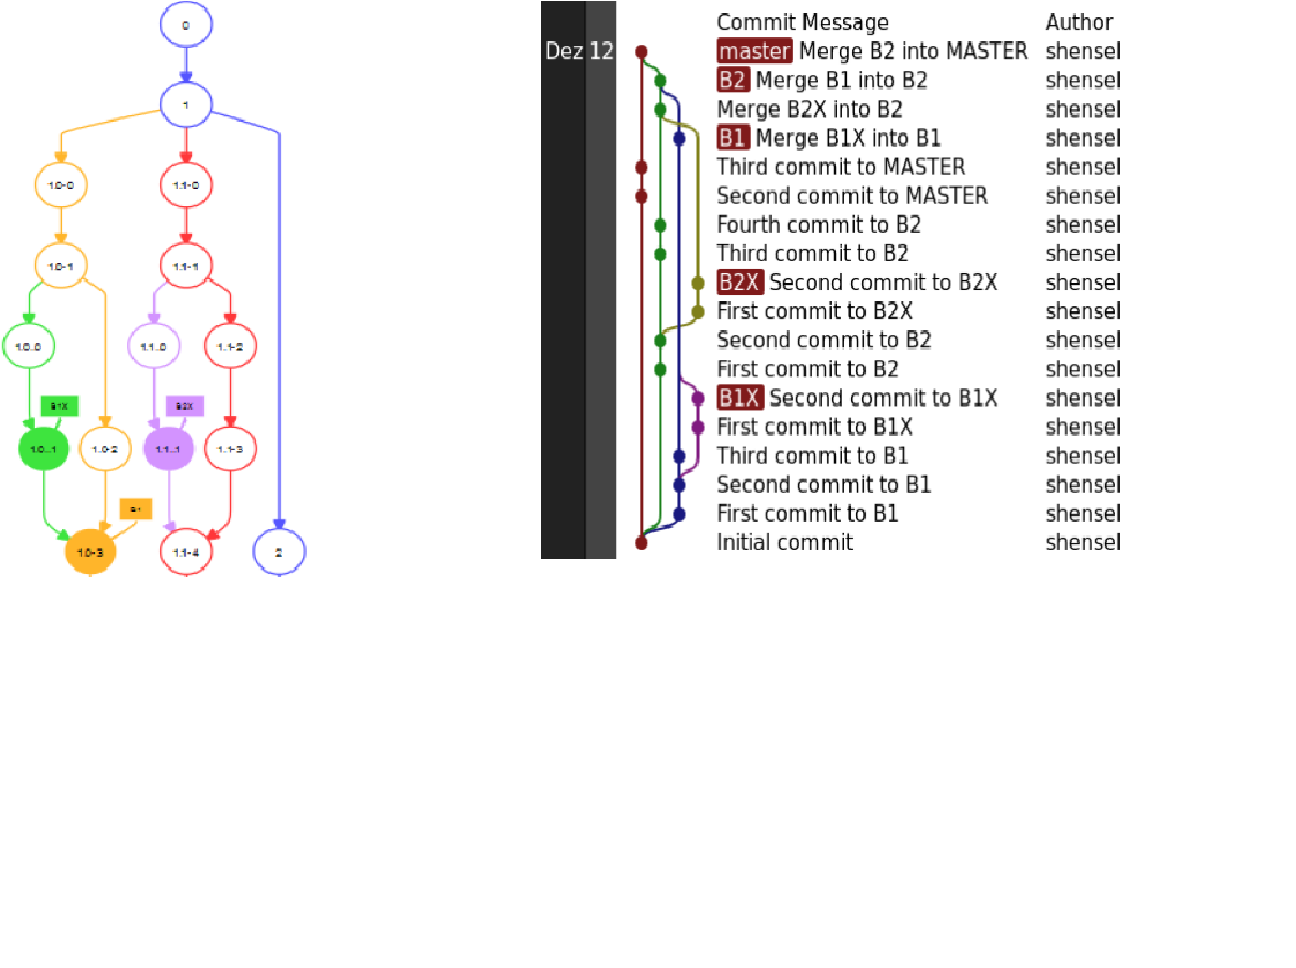
\includegraphics[width=1.2\textwidth]{Vorarbeiten.png}
  \caption[Visualisierungen der vorherigen Gruppen, links Gruppe 2.1 (aus \cite{Gruppe2.1}), rechts Gruppe 2.3 (aus \cite{Gruppe2.3})]{Visualisierungen der vorherigen Gruppen, links Gruppe 2.1, rechts Gruppe 2.3}
  \label{fig:Vorarbeiten}
\end{figure}

Die zweite Visualisierung in \cite{Gruppe2.3} stellt den Graphen mehr an die Seite und stellt mit dem Kommentar zu jedem Commit sowie dem Autor zusätzliche Informationen dar. Die zeitliche Abfolge ist hier ersichtlich, zudem ist eine Einteilung in Monate gegeben. Der Graph wird durch diese Darstellung allerdings relativ klein und der Text dominiert die Visualisierung. Im dargestellten Beispiel sind die Kommentare immer sehr kurz gehalten, dies muss aber nicht zwangsläufig so sein muss, sodass es in dieser Art der Darstellung bei längeren Kommentaren zu Zeilenumbrüchen kommt, was den Graph in die Länge zieht.  

Beide Visualisierungen sind in Abbildung \ref{fig:Vorarbeiten} zu sehen.

\section{Weitere Literatur}
\label{sec:WeitereLiteratur}
\subsection{Git2PROV}
\label{sec:Git2PROV}
In \cite{Git2PROV} wird mit W3C PROV ein neuer Standard eingeführt, um Versionskontrollsysteme wie Git einfacher benutzen und veröffentlichen zu können, zu sehen in Abbildung \ref{fig:Git2PROV}. Dort sind viele Informationen des semantischen Netzes dargestellt, die verschiedenen Arten von Informationen sind durch unterschiedliche Formen dargestellt. So sind die Commits in Rechtecken aufgeführt, die Namen der Autoren in Trapezen, außerdem sind die Kanten mit Spezifizierungen der Beziehungen, in der die Knoten stehen, versehen. Damit bietet dieses Format sehr viele Informationen, ist dabei aber weniger intuitiv und es braucht eine gewisse Einarbeitungszeit, bis damit umgegangen werden kann. Dieses Modell ist eher als Werkzeug für Entwickler gedacht und damit als Vorlage für R43ples nicht geeignet, da hier mehr auf den Anwender eingegangen werden soll, der die wesentlichen Informationen dargestellt haben möchte anstatt einer ausführlichen Beschreibung des semantischen Netzes.

\begin{figure}[htbp] 
  \centering
     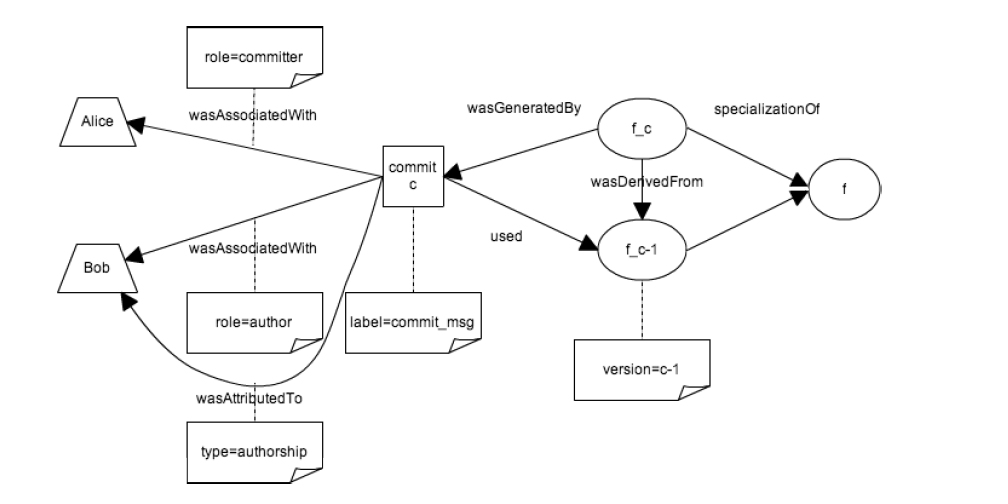
\includegraphics[width=\textwidth]{Git2PROV.png}
  \caption[Darstellung eines Graphen mit Git2PROV, entnommen aus \cite{Git2PROV}]{Darstellung eines Graphen mit Git2PROV}
  \label{fig:Git2PROV}
\end{figure}

\subsection{GitHub Desktop}
GitHub stellt ein Desktop Tool zur Verfügung, in dem ebenfalls der Verlauf der verschiedenen Branches eines Projektes zu sehen ist, dargestellt in Abbildung \ref{fig:GitHubDesktop}. Hier werden für den markierten Commit relativ umfangreiche Informationen angezeigt, es ist genau ersichtlich, was sich im Vergleich zur vorherigen Version geändert hat, außerdem sind die Kommentare der einzelnen Commits samt Benutzerbild des Autors zu sehen. Es wird zwischen Commits und Merges unterschieden und der Zeitverlauf ist durch unterschiedliche Abstände ersichtlich, außerdem wird unter dem Kommentar angezeigt, wie viel Zeit seitdem vergangen ist. Es werden allerdings nur die Commits des markierten Branches angezeigt und dort auch nur die aktuellsten. Dies erhöht die Übersichtlichkeit, insbesondere bei umfangreichen Projekten, die Suche nach einzlnen Commits gestaltet sich aber aufwendiger, auch weil die Knoten keine Beschriftung haben, wodurch eine direkte Zuordnung nicht möglich ist, die Revisionsnummer taucht gar nicht auf.

\begin{figure}[htbp] 
  \centering
     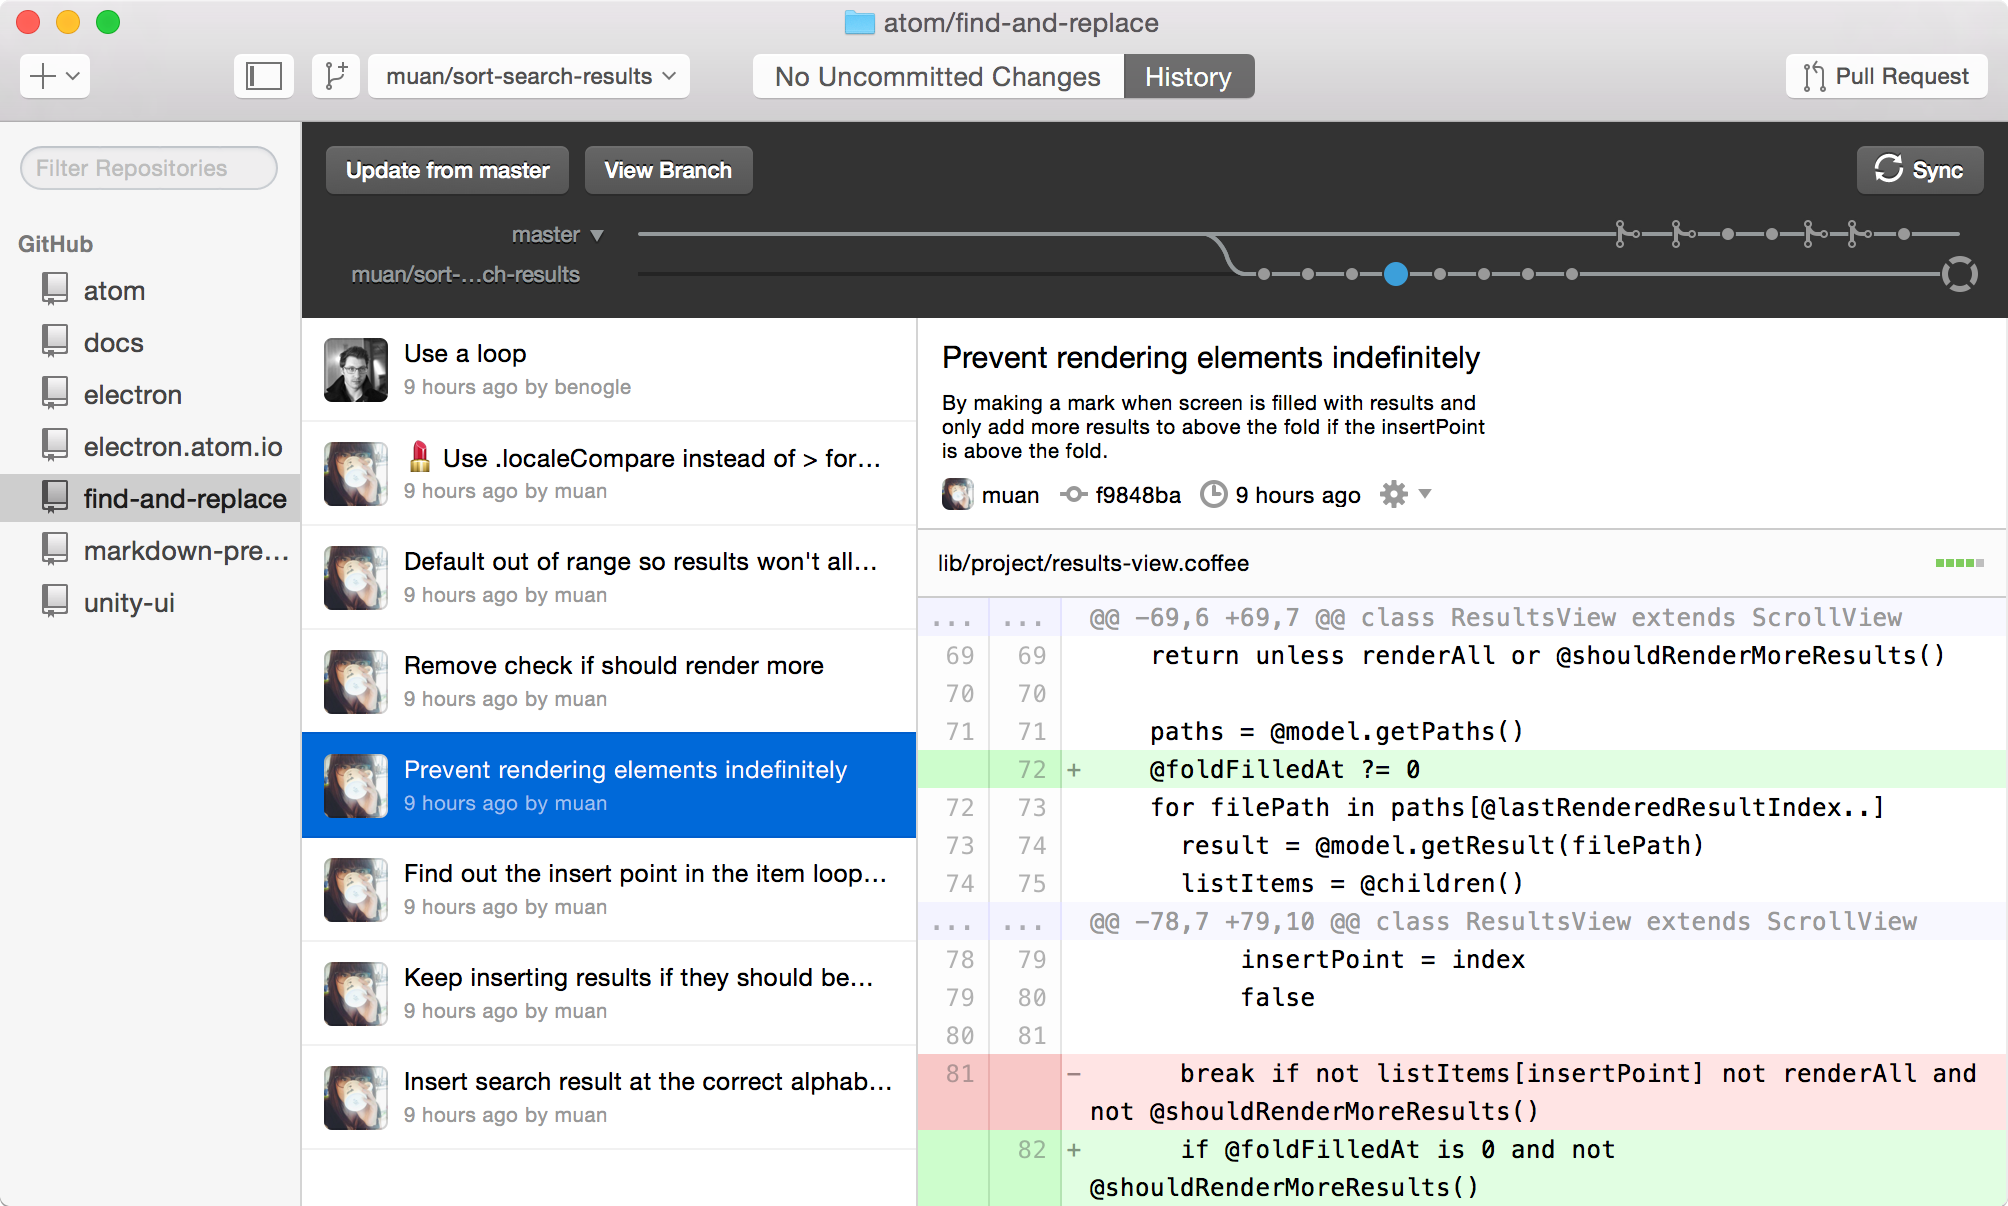
\includegraphics[width=\textwidth]{GitHubDesktop.png}
  \caption[Darstellung eines Graphen mit GitHub Dekstop, entnommen von \GitHubDesktop, abgerufen am 24.11.2015]{Darstellung eines Graphen mit GitHub Desktop}
  \label{fig:GitHubDesktop}
\end{figure}

\chapter{Anforderungsdefinition}
\section{Einleitung}
\subsection{Zielsetzung}
In der vorliegenden Arbeit soll die im vorangegangenen Abschnitt analysierte, vorhandene Visualisierung für das semantische Revisionsverwaltungssystem R43ples erweitert werden, sodass die Inhalte der Changesets der Revisionen sichtbar werden. Der neue Entwurf soll sich dabei gut in die bisherige HTML-Oberfläche integrieren und gut skalieren in Bezug auf die Größe der Changesets.

\subsection{Produktziele}
Die Entwicklung soll als Fork auf GitHub durchgeführt werden, als Implementierungssprache ist Javascript vorgesehen. Es existiert eine HTML-Oberfläche, die weiter verwendet werden soll.

\section{Allgemeine Beschreibung}
\subsection{Produktumgebung}
Revisionsverwaltungssysteme werden im Allgemeinen vorwiegend auf Desktop-PCs oder Laptops verwendet, evtl. auch auf Tablets. Das Produkt soll also für eine Nutzung an einem Bildschirm im Querformat optimiert werden. Deshalb soll der Graph, statt wie in der bisherigen Visualisierung von oben nach unten, von links nach rechts angezeigt werden, um den Platz optimal auszunutzen und so auch lange Graphen ohne Scrollen darstellen zu können. Für zusätzliche Informationen bietet sich dadurch am unteren Bildschirmrand Platz, am oberen Rand soll eine Zeitleiste angezeigt werden.

\subsection{Benutzereigenschaften}
Anders als die in Abschnitt \ref{sec:Git2PROV} beschriebene Visualisierung, die eher für Entwickler gedacht ist, ist R43ples für Anwender gedacht, die keine ausführliche Darstellung des semantischen Netzes, sondern eine übersichtliche Visualisierung der wichtigen Informationen benötigen. 

\subsection{Qualitätsanforderung}
\begin{enumerate}[Q1]
\item Erfüllen der Konventionen aus Abschnitt \ref{sec:Richtlinien}:
	\begin{enumerate}[Q1.1]
		\item Alle Kanten als gerade Linien zeichnen.
		\item Kreuzungen von Graphen nur an Knoten.
		\item Minimierung der Fläche und der Gesamtkantenlänge
	\end{enumerate}
\end{enumerate}

\subsection{Produktfunktion}
\begin{enumerate}[F1]
\item Übersichtlichkeit und Lesbarkeit der Graphen durch Einhalten der Richtlinien und Kriterien aus Abschnitt \ref{sec:Richtlinien}, sowie durch Beschränken auf die entscheidenden Informationen
\item Automatische Anordnung der Revisionen nach Zeitpunkt des Commits und der Verbindungen
\item Hervorheben des Master Branches, kennzeichnen der Branches mit Namen und Gruppierung durch einheitliche Farbgebung
\item Direkt dargestellt werden soll zudem die Revisionsnummer
\item Hinzufügen weiterer Informationen wie Changeset oder Kommentar durch Mouseover bzw. Klicken
\item Darstellung der zusätzlichen Informationen am unteren Bildschirmrand
\item Hinzufügen einer Zeitleiste am oberen Bildschirmrand
\end{enumerate}

\subsection{Allgemeine Einschränkungen und Randbedingungen}



\chapter{Gestaltungsentwurf und Implementierung}
Ideen:
\begin{itemize}
\item Mouseover für mehr Informationen
\item Evtl. durch Klick dauerhaftes Hinzufügen der Informationen
\item Show und Hide Haken
\item evtl Änderung der Form auf Rechteck, um mehr Platz für zusätzliche Informationen zu erhalten
\item Commits und Tags sollen weiterhin klar unterscheidbar sein, evtl. durch Farbe
\item Vermeiden von Kreuzungen
\item Ausgleich zwischen Information und Übersichtlichkeit finden
\item Neuestes nach oben
\item Evtl. Master in der Mitte, alles andere drum herum anordnen
\item Evtl. Einfügen einer Suche
\item Entscheidendes Ziel der zusätzlichen Informationen: Schnelles Finden der Version, die wiederhergestellt werden soll
\item add und remove durch Symbol darstellen
\item Mit Klick/Mouseover Informationen, was geaddet bzw. removed wurde
\item Sortierung nach Datum? Evtl. auch grobe Zeiteinteilung
\item Bei Klick werden Add und Delete Sets mit angezeigt (was wurde hinzugefügt, was wurde gelöscht)
\item Anzeige in Fenster am unteren Bildschirmrand
\item Zeitleiste
\end{itemize}

\bibliography{MMST}
\bibliographystyle{gerabbrv}
\listoffigures

\end{document}
